% !TeX root = ../Notizen.tex

\section*{Aufgabe 4: Kepler-Ellipsen}
Das Programm aus Aufgabe 1 wird jetzt verwendet, um die Planetenbahnen zu bestimmen.
Dazu wird die Zentralkraft verwendet
\begin{align}
	\frac{1}{m}\vec{F}(\vec{r})=-G\frac{\vec{r}}{r^3}~,
\end{align}
wobei $G=1$ gesetzt wird.
\subsection*{a)}
Hier werden zwei Teilchenbahnen für die Masse $m=\SI{1}{kg}$ erstellt.
Für das erste Teilchen werden die Startvektoren 
\begin{align}
	\vec{r}_1=
	\begin{pmatrix}
		1,0\\0,0\\0,0
	\end{pmatrix}\text{ und }
	\vec{v}_1=
	\begin{pmatrix}
		-0,5\\1,0\\0,0
	\end{pmatrix}
\end{align}
verwendet und für den zweiten
\begin{align}
	\vec{r}_2=
	\begin{pmatrix}
		1,0\\0,0\\0,0
	\end{pmatrix}\text{ und }
	\vec{v}_2=
	\begin{pmatrix}
		-0,1\\1,0\\0,0
	\end{pmatrix}.
\end{align}
Die resultierenden Bahnen sind in \cref{fig:Bahn} dargestellt.
Diese wurden mit $h=0,01$ und $t=\SI{10}{s}$ erstellt.
In \cref{fig:Bahn2} ist die Bahn für größere Breiten dargestellt.
Es lässt sich erkennen, dass die Ellipse erst eckiger wird und sich später wie eine Spirale zum Ursprung bewegt.
Für kleine Anfangsgeschwindigkeiten fällt das Teilchen in den Ursprung und bekommt eine starke Beschleunigung und läuft dann weg, wie in \cref{fig:Bahn3} dargestellt.\\

\begin{figure}[H]
	\begin{subfigure}[c]{0.5\textwidth}
		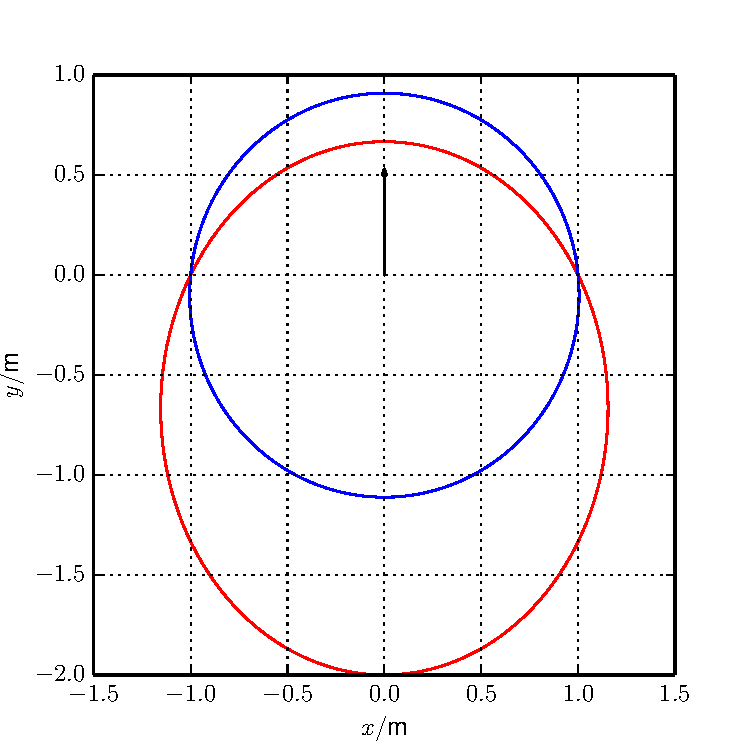
\includegraphics[width = \textwidth]{../Plots/Plot_4_A_1.pdf}
		\caption{2 simulierte Planetenbahnen sowie der Lenz-Runge-Vektor.\label{fig:Bahn}}
	\end{subfigure}
	\begin{subfigure}[c]{0.5\textwidth}
		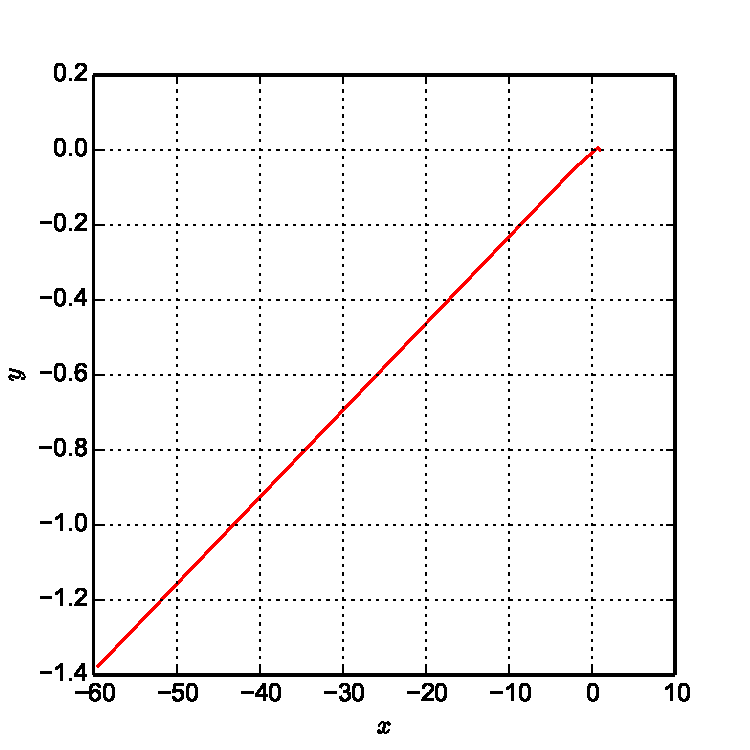
\includegraphics[width = \textwidth]{../Plots/Plot_4_A_5.pdf}
		\caption{Verhalten der Planetenbahn für kleine Anfangsgeschwindigkeiten. \label{fig:Bahn3}}
	\end{subfigure}
	\begin{subfigure}[c]{0.5\textwidth}
		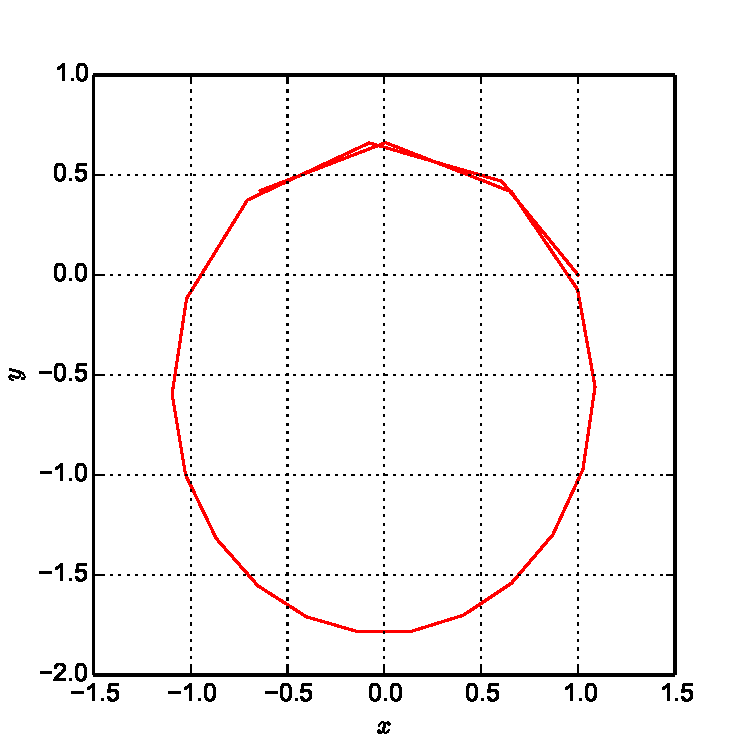
\includegraphics[width = \textwidth]{../Plots/Plot_4_A_3.pdf}
		\caption{Planetenbahn für $h=0,5$.}
	\end{subfigure}
	\begin{subfigure}[c]{0.5\textwidth}	
		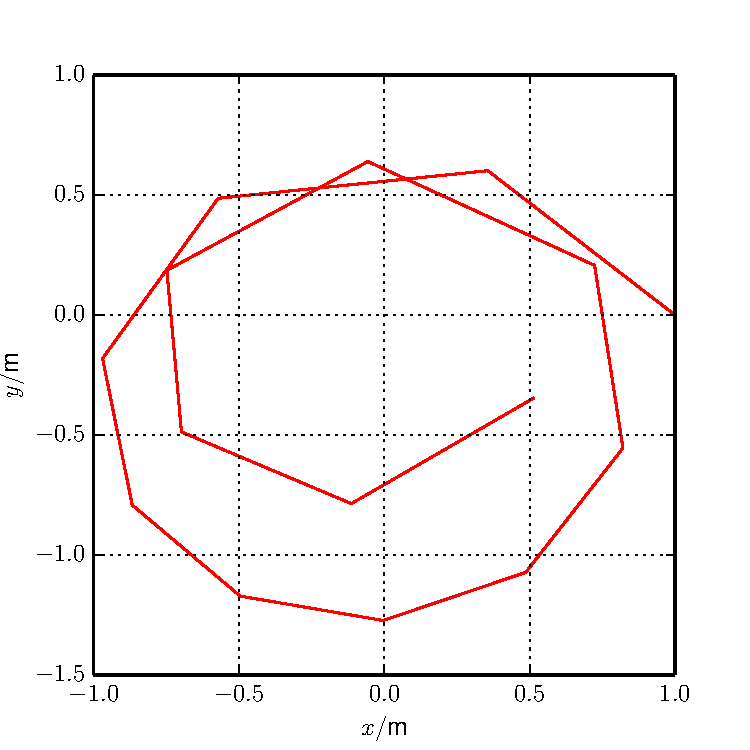
\includegraphics[width = \textwidth]{../Plots/Plot_4_A_4.pdf}
		\caption{Planetenbahn für $h=0,7$.\label{fig:Bahn2}}
	\end{subfigure}\\
\end{figure}

\subsection*{b)}
Als nächstes soll überprüft werden, ob die Energie in dem System erhalten ist.
Sie ist definiert als
\begin{align}
	E:=\frac{1}{2}v^2-\frac{mG}{r}
\end{align}
Hier wird wieder die Energiedifferenz $\Delta E$ für unterschiedliche Zeiten $t$ betrachtet.
Aus ihrer Größenordnung von $10^{-6}$ ist ersichtlich, dass die Energie wieder im Wesentlichen erhalten ist.
In \cref{fig:Energie} ist die Energiedifferenz $\Delta E$ gegen die Zeit $t$ aufgetragen.
\begin{figure}[H]
	\centering
	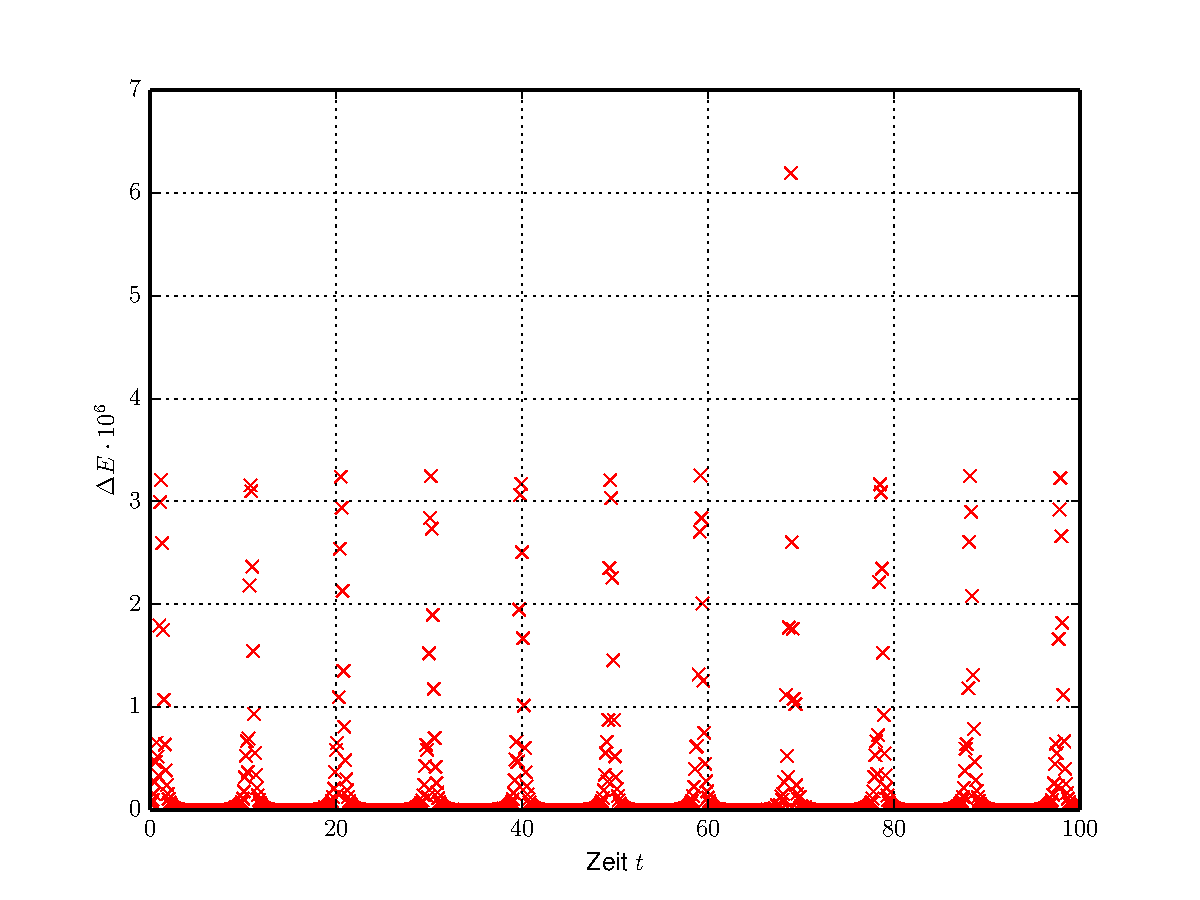
\includegraphics[width = \textwidth]{../Plots/Plot_4_Energie.pdf}
	\caption{Energiedifferenz $\Delta E$ für verschiedene Zeiten $t$.\label{fig:Energie}}
\end{figure}
Analog lässt sich dieselbe Aussage für den Drehimpuls
\begin{align}
\vec{L}=\vec{r}\times\vec{p}=\vec{r}\times m\vec{v}
\end{align}
treffen, dessen Betrag in \cref{fig:Dreh} ebenfalls gegen die Zeit $t$ aufgetragen ist.
\begin{figure}[H]
	\centering
	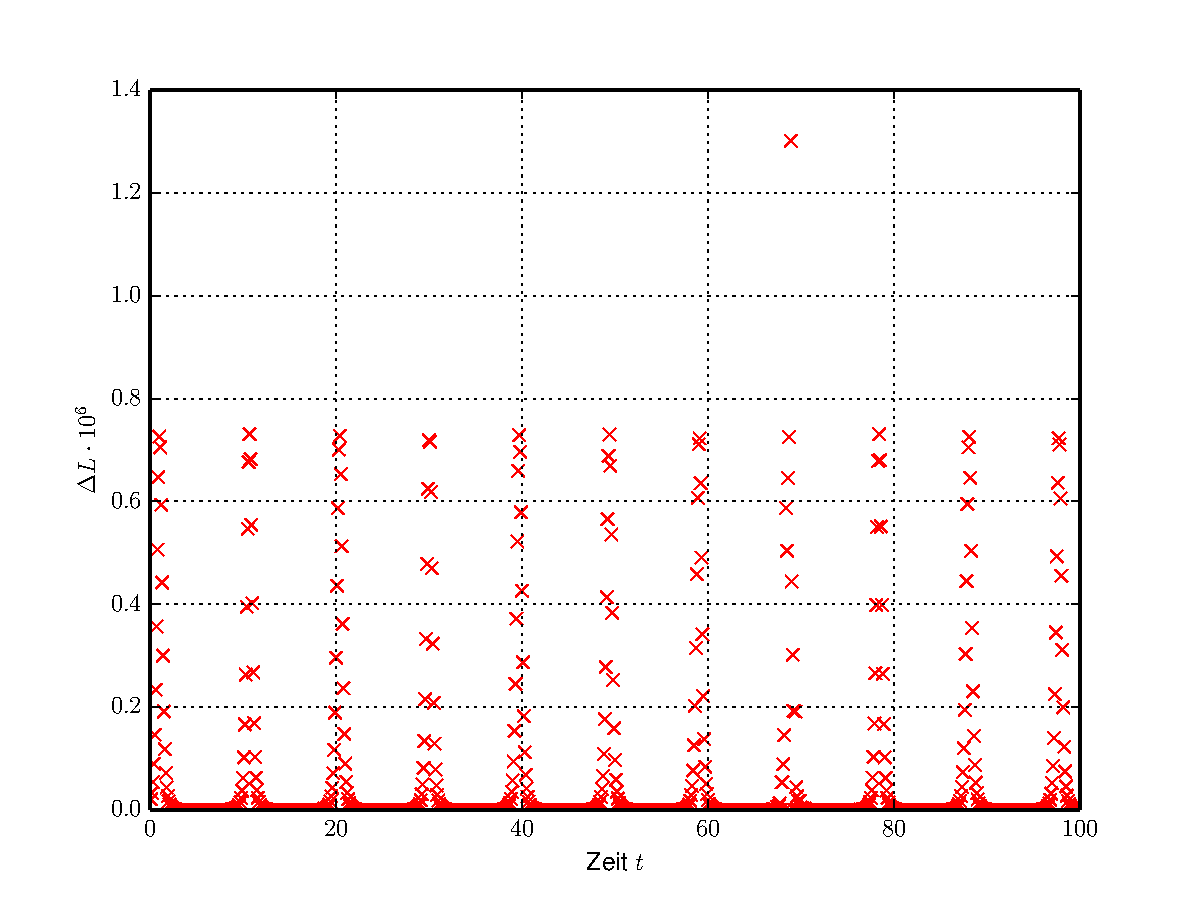
\includegraphics[width = \textwidth]{../Plots/Plot_4_Dreh.pdf}
	\caption{Drehimpulsdifferenz $\Delta L$ für verschiedene Zeiten $t$.\label{fig:Dreh}}
\end{figure}
Weiter soll noch das 3. Kepler-Gesetz überprüft werden, nach dem gilt:
\begin{align}
	\frac{a_1^3}{T_1^2}=\frac{a_2^3}{T_2^2}
\end{align}
Darin sind $a_i$ die Länge der großen Halbachsen und $T_i$ die Umlaufzeiten, für 2 verschiedene Bahnen.
Bestimmt werden die Werte aus \cref{tab:kepler}. Dabei werden für die Umlaufzeit die Werte verwendet, bei denen die Bahn in einen Bereich von $|x-x_0|<10^{-1}$ und $|y-y_0|<10^{-1}$ zum Ausgangspunkt kamen. Dabei wurde der Mittelwert von 8 Datenpunkten berechnet. Für die große Halbachse wird der größte Abstand zweier Punkte auf den Bahnen verwendet. 
Daraus folgt
\begin{align}
	\left|\frac{a_1^3}{T_1^2}-\frac{a_2^3}{T_2^2}\right|\approx 0,07005
\end{align}
Dabei werden die Planetenbahnen wie in \cref{fig:Bahn} dargestellt verwendet.
\begin{table}[h!]
	\centering
	\begin{tabular}{c|c|c}
		Umlaufzeit & Länge der großen Halbachse&$a^3/T^2$ \\\hline
		9,86771 & 2,66653 & 0,19472\\
		5,58021 & 2,02019 & 0,26477
	\end{tabular}\caption{Ergebnis der Umlaufzeiten- und Halbachsenberechnung.\label{tab:kepler}}
\end{table}\\
Wegen der größeren numerischen Ungenauigkeiten lässt das Ergebnis trotzdem noch den Schluss zu, dass das 3. Kepler-Gesetz näherungsweise gilt.

\subsection*{c)}
Genau wie in Aufgabenteil b) wird nun die Erhaltung des Lenz-Runge-Vektors $\vec{\Lambda}$ überprüft.
Dessen Betrag ist in \cref{fig:LR} wiederum gegen die Zeit $t$ aufgetragen.
Er berechnet sich nach
\begin{align}
\vec{\Lambda}=\frac{1}{Gm}\vec{p}\times\vec{L}-\frac{\vec{r}}{r}
=\underbrace{\vec{v}\times\left(\vec{r}\times\vec{v}\right)}_{(\vec{v}\cdot\vec{v})\vec{r}-(\vec{v}\cdot\vec{r})\vec{v}}-\frac{\vec{r}}{r}~.
\end{align}
\begin{figure}[H]
	\centering
	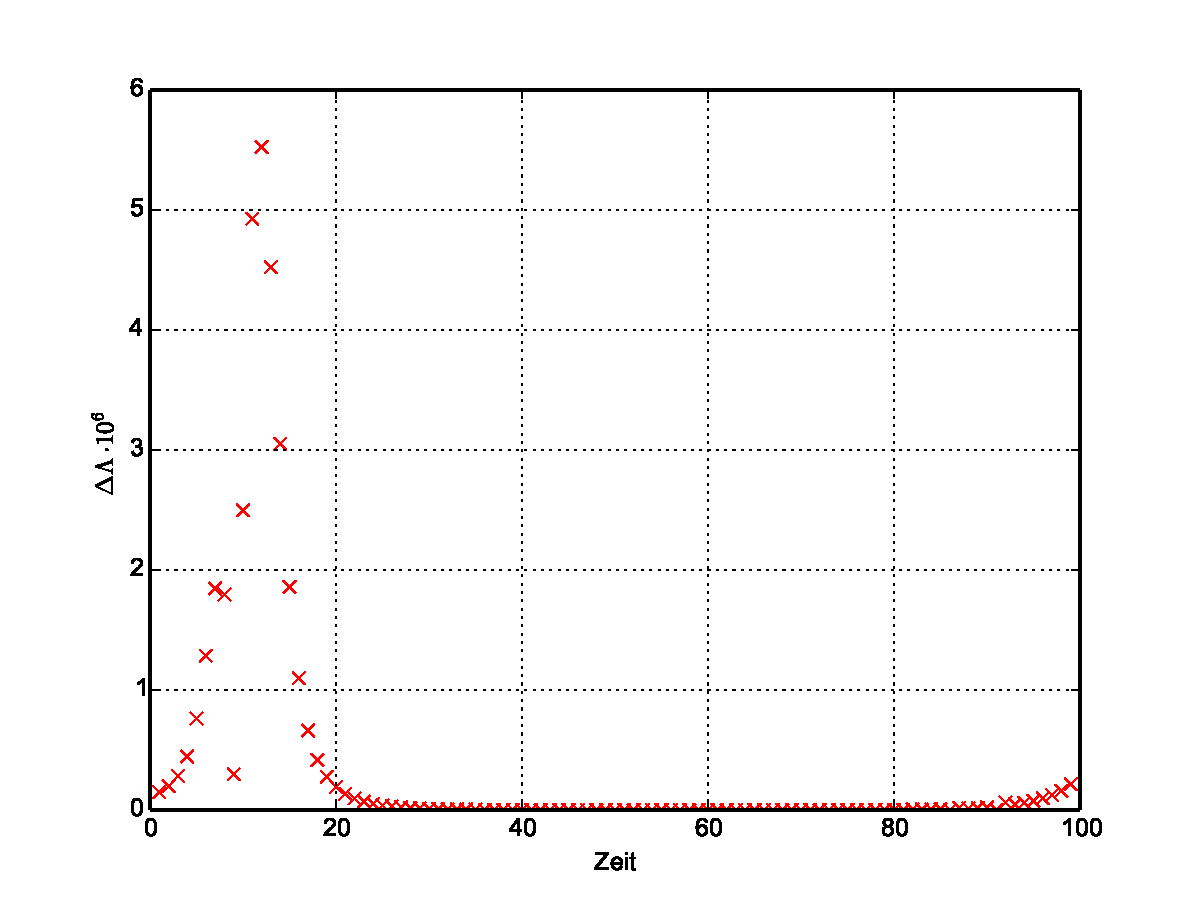
\includegraphics[width = \textwidth]{../Plots/Plots_4_LR.pdf}
	\caption{Änderung des Betrages des Lenz-Runge-Vektor $\Lambda$ für verschiedene Zeiten $t$.\label{fig:LR}}
\end{figure}
Auffällig ist hier das Maximum um etwa \SI{10}{s}.
Trotzdem lässt sich die Aussage treffen, dass auch der Lenz-Runge-Vektor im Wesentlichen erhalten ist.\\
In \cref{fig:Bahn} ist die Richtung des Lenz-Runge-Vektors eingezeichnet.

\subsection*{d)}
Um die Fehler und Stabilität der Integration zu testen, werden $N$ Runge-Kutta-Schritte gemacht und anschließend die Geschwindigkeit $\vec{v}$ umgekehrt.
Vom erreichten Punkt aus werden dann $N$ Runge-Kutta-Schritte in die entgegengesetzte Richtung gemacht.
Nun werden der erreichte Punkt und die dortige Geschwindigkeit mit dem Ausgangspunkt und der Ausgangsgeschwindigkeit verglichen.
Abgesehen von kleinen numerischen Abweichungen stimmen diese gut überein.
(Siehe Ausgabe des Programms)

\subsection*{e)}
In diesem Aufgabenteil sollen die Bahnen für Potentiale der Art
\begin{align}
	V(\vec{r})=-\frac{mG}{r^\alpha}
\end{align}
untersucht werden. 
Dabei werden speziell die betrachtet mit $\alpha=0,1$ und $\alpha=1,1$.
Es lässt sich erkennen, dass die Teilchenbahnen anfangen zu rotieren.
Dies hat für den Lenz-Runge-Vektor die Konsequenz, dass er keine Erhaltungsgröße mehr ist.
Die Teilchenbahnen sind in \cref{fig:E1} und \cref{fig:E2} dargestellt. Es sind ebenfalls je 2 Lenz-Runge-Vektoren eingezeichnet.

\begin{figure}[H]
	\centering
	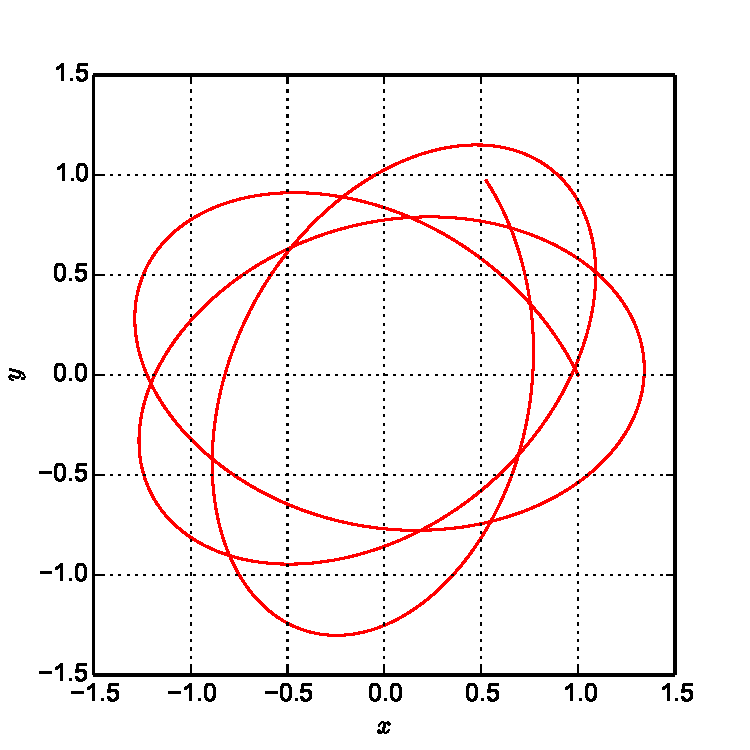
\includegraphics[width = \textwidth]{../Plots/Plot_4_E_1.pdf}
	\caption{Eine Teilchenbahn für das Potential $\propto\frac{1}{r^{0,9}}$.\label{fig:E1}}
\end{figure}

\begin{figure}[H]
	\centering
	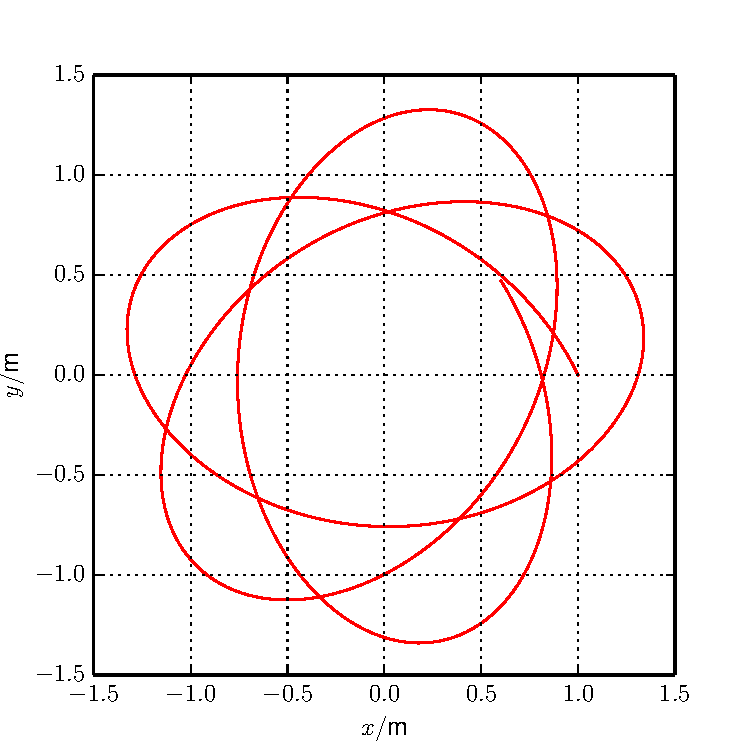
\includegraphics[width = \textwidth]{../Plots/Plot_4_E_2.pdf}
	\caption{Eine Teilchenbahn für das Potential $\propto\frac{1}{r^{1,1}}$.\label{fig:E2}}
\end{figure}